\documentclass{article}
\usepackage{graphicx}
\graphicspath{{./images/}}

\usepackage{lipsum}
\usepackage{fancyhdr}
\pagestyle{fancy}
\lhead{\centering{\Large \textbf{Tushar Patil}}}
\cfoot{center of the footer!}
\renewcommand{\headrulewidth}{0.5pt}
\renewcommand{\footrulewidth}{0.5pt}

\begin{document}
	
	\begin{minipage}{2in}
	H.No: 918
	\end{minipage}
	\hfill
	\begin{minipage}{2.25in}
	Contact: 8867514363
	\end{minipage}

	
	\begin{minipage}{2in}
	Sambhaji Nagar,
	\end{minipage}
	\hfill
	Email-id:patil.tushar1998@gmail.com
	
	\begin{minipage}{2in}
	Macche, Belgavi
	\end{minipage}
	
	\begin{minipage}{2in}
	Belgavi - 590014
	\end{minipage}

	\begin{minipage}{2in}
	Karnataka
	\end{minipage}

	\begin{figure}[h!]
		\hfill
		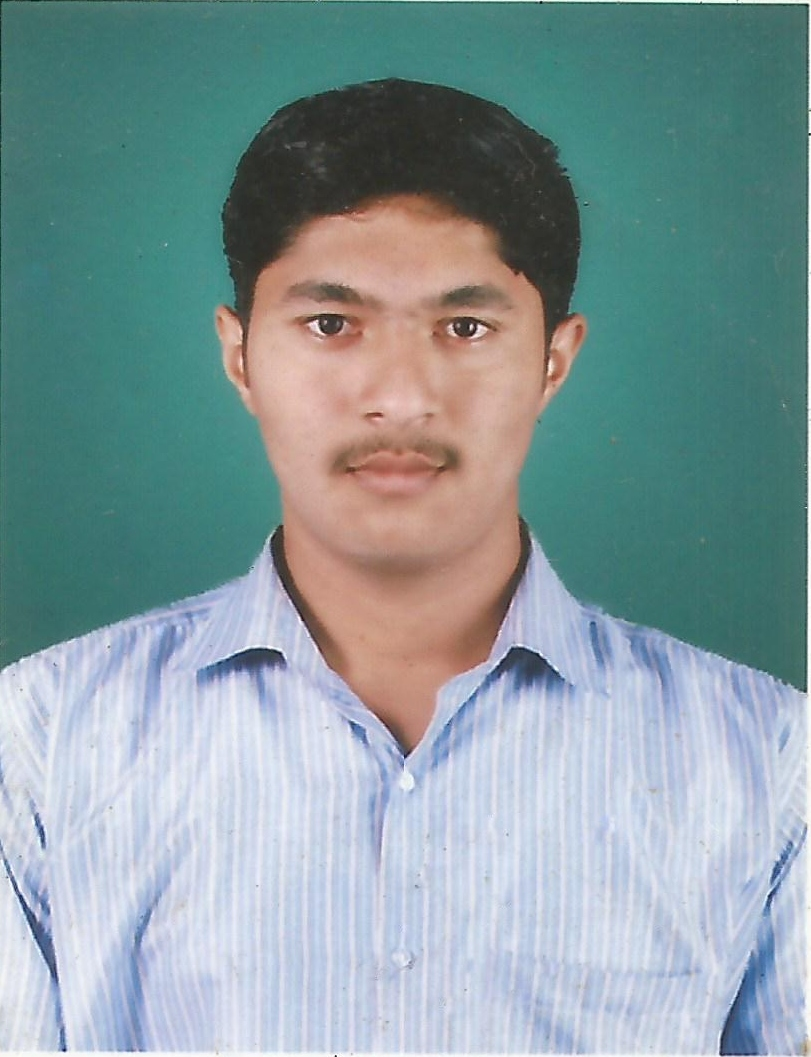
\includegraphics[scale = 0.6]{profilepic.jpg}
		\label{image_1} % Label is used for referencing
	\end{figure}
	
		
\large \textbf{OBJECTIVE:}
	\texttt{	
	To use Computer Science training in Software Development for designing and implementing Applications in various platforms to solve various problems}.
\vspace{\baselineskip}
	
	\large \textbf{EDUCATION}:
	
	\begin{tabular}{|c|c|c|c|c|}
	\small Degree & \small College/School & \small University & \small Passing Year & \small Pass Percentage \\
		\hline
		\footnotesize  B.E.(CSE)  & \footnotesize Jain College of Engineering & \footnotesize Visvesvaraya Technological University & \footnotesize 2020 & \footnotesize 7.56(till 5th Sem) \\
		\footnotesize PUC(Science) & \footnotesize MGV-PU College & \footnotesize Karnataka PU Board & \footnotesize 2016 &\footnotesize 74\%  \\
		\footnotesize SSLC & \footnotesize Dnyan Prabodhan Mandir & \footnotesize ICSE & \footnotesize 2014 & \footnotesize 75 \%  \\

\vspace{\baselineskip}
	\end{tabular}
\\
	\large \textbf{Projects}:
	\begin{enumerate}
		\item Blind Calculator | Android App
		\item Online-Quiz | Web Application
		\item Line Following Robot | E-Yantra 2018
		\item Scanner | Android Application
		
		\vspace{\baselineskip}
	\end{enumerate}
	\large \textbf{Training And Internships:}	
	None
	

\end{document}